\graphicspath{{content/chapters/5_design/figures/}}
\chapter{Design}
\label{chp:design}

This chapter outlines the core design components that form the foundation of the speech enhancement system. It begins by addressing the challenge of handling variable-length audio inputs, a key consideration for batch-based model training. The latter and more substantial section focuses on the design of the machine learning architectures used in this project. Detailing each model's structure and the reasoning behind their implementation for speech enhancement.

\section{Variable Length Handling}
\label{sec:variable_length_handling}

For this project, only the clean and noisy pairs of audio files from the dataset are required. The transcript text files are ignored, as they are not relevant to the task. However, it is worth noting that such transcripts are highly valuable in other applications, such as training text-to-speech or speech recognition models. As highlighted in the dataset analysis in Section~\ref{sec:dataset_exploration}, the audio files vary in length. This poses a challenge for model training, as batch processing requires input tensors to have consistent dimensions.

To address this, several algorithms for handling variable-length audio inputs were explored. The most basic approach involves padding each audio file to match the length of the longest sample in the batch, typically by appending zeros to the end of shorter files. While this method is simple, it has significant drawbacks. Excessive padding introduces unnecessary data that may act as noise during training, making it harder for the model to learn effectively. The greater the variation in input lengths, the more padding is required. Which can negatively impact overall training performance.

\begin{figure}[h]
    \centering
    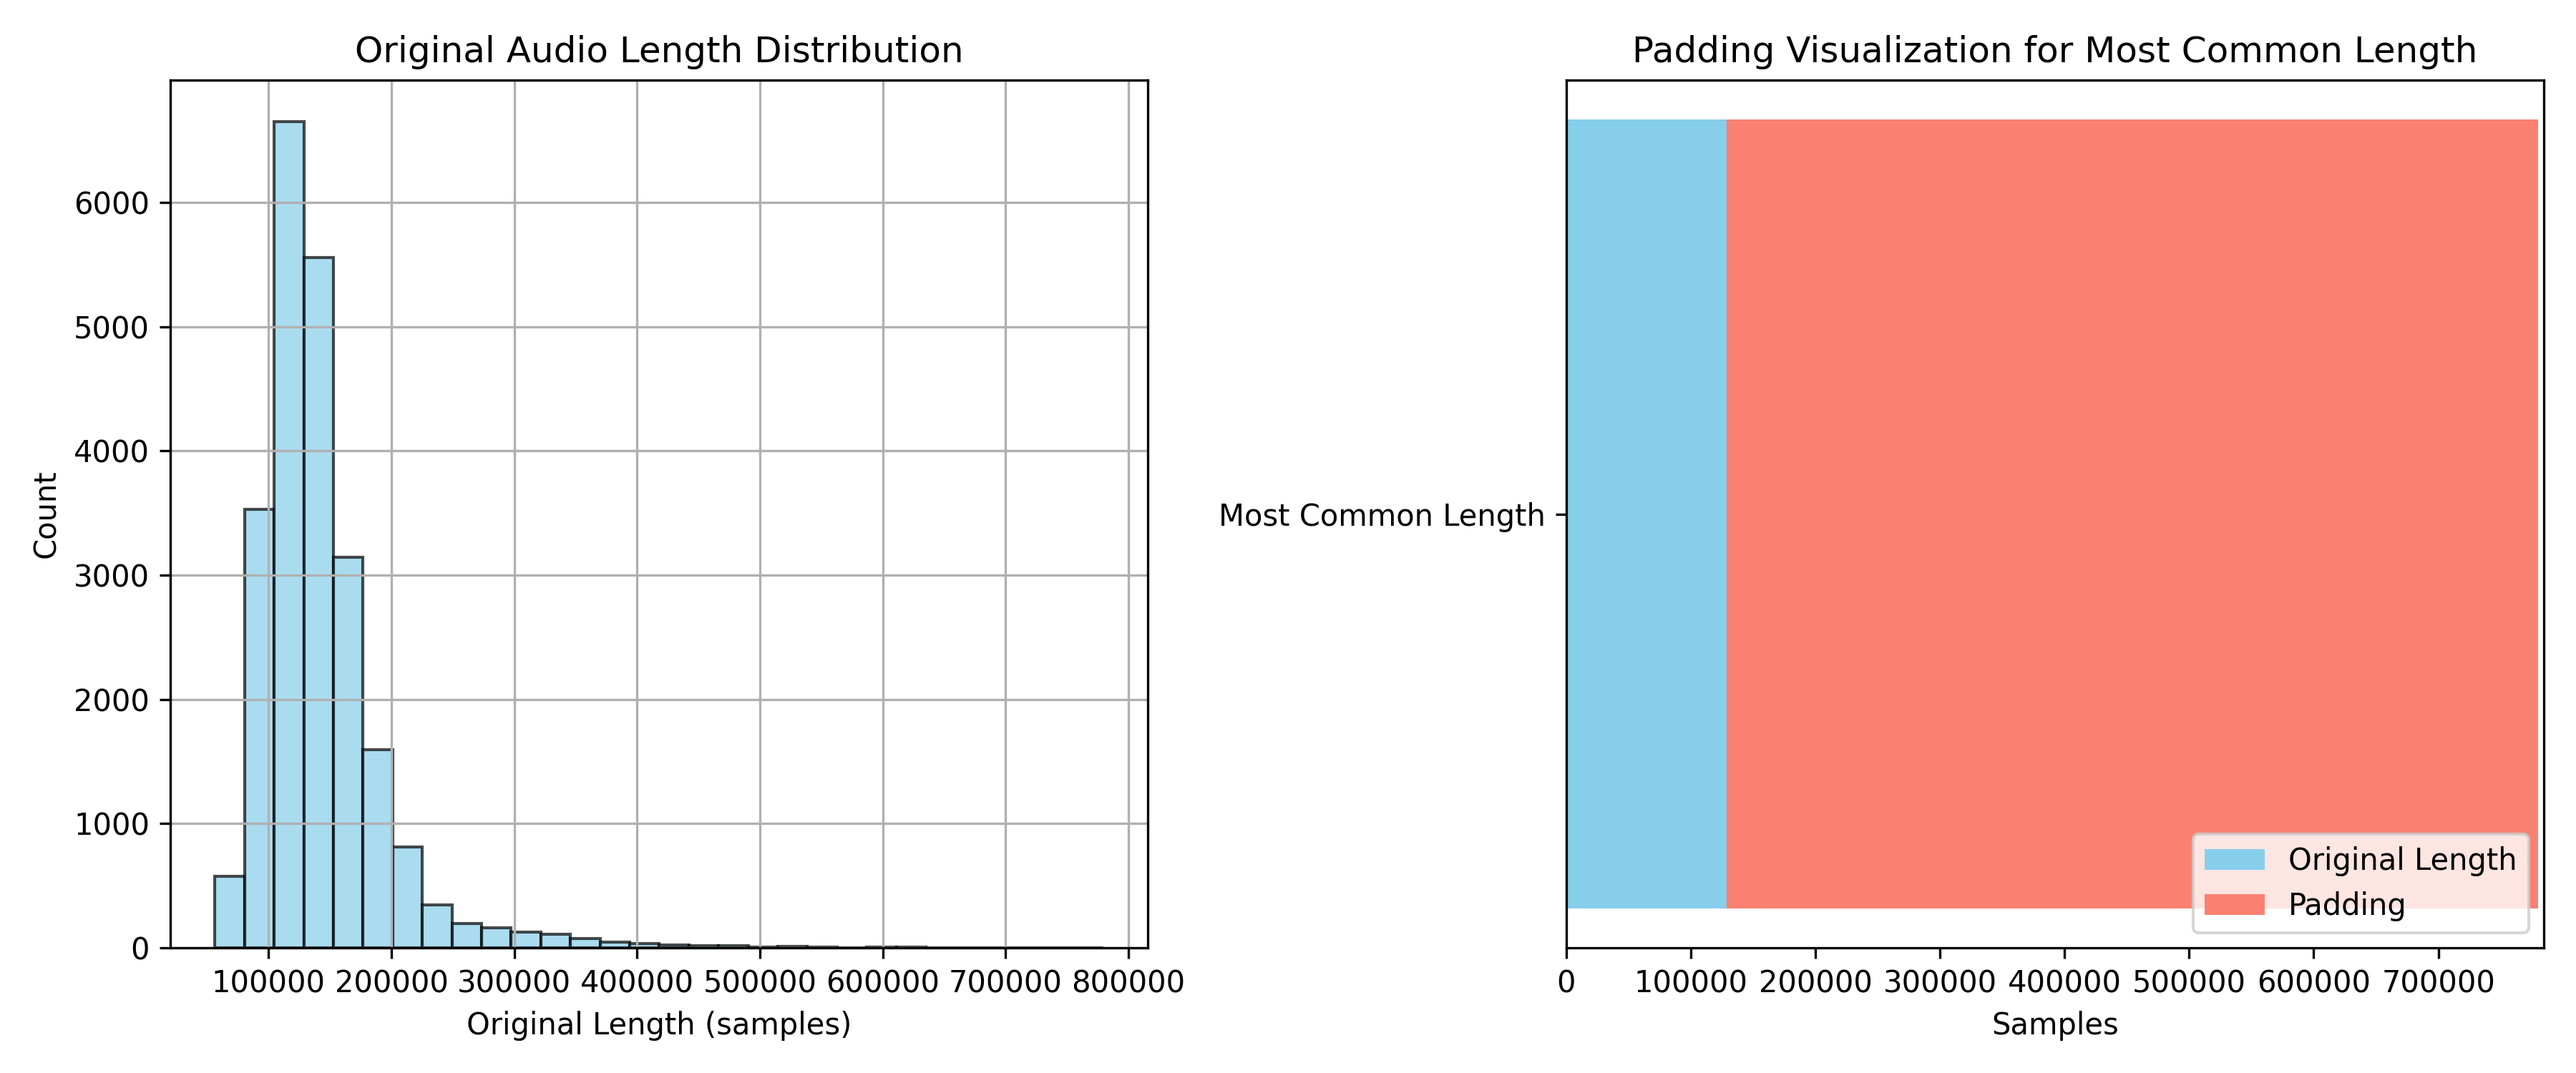
\includegraphics[width=\textwidth,keepaspectratio]{max_padding.png}
    \caption{\label{fig:max_padding}Illustration of maximum-length padding.}
\end{figure}

As shown in Figure~\ref{fig:max_padding}, the most common audio length is padded so heavily that the padding exceeds the actual content. This is far from ideal. To mitigate this issue, three different padding strategies were used. Each method aims to reduce the impact of excessive padding on model performance.

The first method is \textit{Static Bucketing}, which essentially groups audio files into predefined fixed-length buckets. Allowing the grouped files to require less unnecessary padding. The second method, \textit{Dynamic Bucketing}, builds on this by creating buckets dynamically based on the distribution of audio lengths, offering a more adaptive grouping approach. The third and final method introduced in Section~\ref{sec:distortion_free_handling}. PTO is a more sophisticated approach that combines padding and truncating to ensure that the minimum distortion is introduced to the data.

All three methods were implemented for testing and evaluation. Their role in the system design is critical, as they help ensure that the model can learn effectively without being hindered by dimensional mismatches or excessive zero-padding. Further details on their implementations are provided in Chapter~\ref{chp:implementation}, and their impact on model performance is discussed in Chapter~\ref{chp:evaluation}.

\section{Model Architecture}
\label{sec:model_architecture}

The model architecture forms the core of the system design, determining how the input is processed, how latent features are transformed, and how the output is reconstructed. The modular project structure facilitates the exploration of a range of neural network models, starting with a simple baseline and progressing to more advanced designs. The main concept of autoencoders for speech enhancement models has already been introduced in Section \ref{sec:autoencoders}. All models operate on spectrogram representations of audio, where the real and imaginary components are concatenated to form a two-channel input. Each network outputs a similarly formatted spectrogram.

Initially, all models included a \texttt{Tanh} activation function at the output layer to constrain values within the range \([-1, 1]\), assuming this would promote numerical stability during the inverse STFT reconstruction. However, during evaluation, it was observed that this constraint suppressed amplitude dynamics and negatively impacted denoising performance across all models. As a result, the \texttt{Tanh} activation was removed from the design of all model outputs. This decision is discussed further in the \ref{sec:tanh_removal}, where the comparative results highlight the improvements achieved by this change.

\subsection{Convolutional Neural Network (CNN)}
\label{sec:cnn}

The CNN model implemented in this project serves as the baseline architecture. Its design follows a widely used encoder-decoder structure. The model operates on concatenated real and imaginary components of the spectrogram, processed as a two-channel input. Its straightforward structure makes it suitable for benchmarking and for validating the core pipeline before exploring more advanced architectures.

The first entry point in the forward pass of the model is the encoder. The encoder consists of three convolutional layers, each followed by a PReLU activation function. Each convolution uses a \(3 \times 3\) kernel. The network begins with 2 input channels and progressively increases to 128 channels. The encoder's role is to reduce the spatial dimensions of the input while increasing the number of feature channels.

\begin{figure}[h]
    \centering
    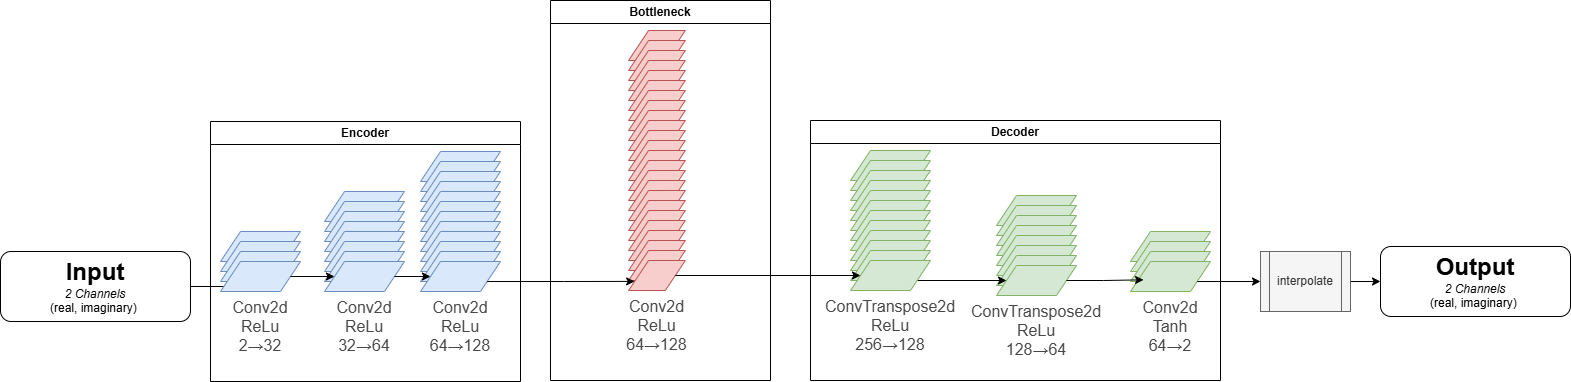
\includegraphics[width=\textwidth,keepaspectratio]{cnn.png}
    \caption{\label{fig:cnn}Basic CNN architecture.}
\end{figure}

The output of the encoder is passed to a bottleneck layer, which further transforms the feature space without altering its spatial resolution. In this implementation, the bottleneck consists of a single \(3 \times 3\) convolutional layer that increases the number of channels from 128 to 256, followed by a ReLU activation. This design deepens the network and allows for more complex feature extraction. Since the bottleneck is not part of the downsampling or upsampling path, it also encourages the decoder to learn a more challenging mapping from latent space back to the input resolution.

The decoder reconstructs the spectrogram from the transformed features using a three-stage transposed convolutional block. It includes two transposed convolutional layers that upsample the spatial dimensions, reversing the compression performed by the encoder. Each is followed by a ReLU activation. A final standard \(3 \times 3\) convolutional layer reduces the channel count from 64 to 2, corresponding to the real and imaginary parts of the output spectrogram. To ensure output consistency, bilinear interpolation is applied to match the original input resolution prior to splitting the output into its two channels.

While simple, this model plays a critical role in establishing a baseline performance level. It ensures that the overall system functions correctly while providing a reference point for evaluating the impact of architectural modifications. The CNN model is straightforward to implement and interpret, making it a suitable starting point for benchmarking and guiding the development of more sophisticated architectures introduced in subsequent sections.

\subsection{Convolutional Encoder Decoder (CED)}
\label{sec:ced}

The Convolutional Encoder Decoder (CED) architecture implemented in this project is based on the design proposed by Park and Lee~\cite{park2017acoustic}, as reviewed in Section~\ref{sec:fcns}. The model follows a symmetric encoder-decoder structure, operating on complex spectrograms represented as two-channel inputs (real and imaginary concatenated along the channel dimension).

The encoder is composed of five convolutional blocks. Each block consists of a convolutional layer with a tall vertical kernel, batch normalization, a ReLU activation function, and a \(2 \times 1\) max pooling operation. The vertical kernel sizes decrease from \(13 \times 1\) to \(5 \times 1\) across layers, preserving frequency resolution while downsampling the temporal dimension. The number of channels increases progressively from 12 to 32, enabling richer feature representations as the input is compressed.

\begin{figure}[h]
    \centering
    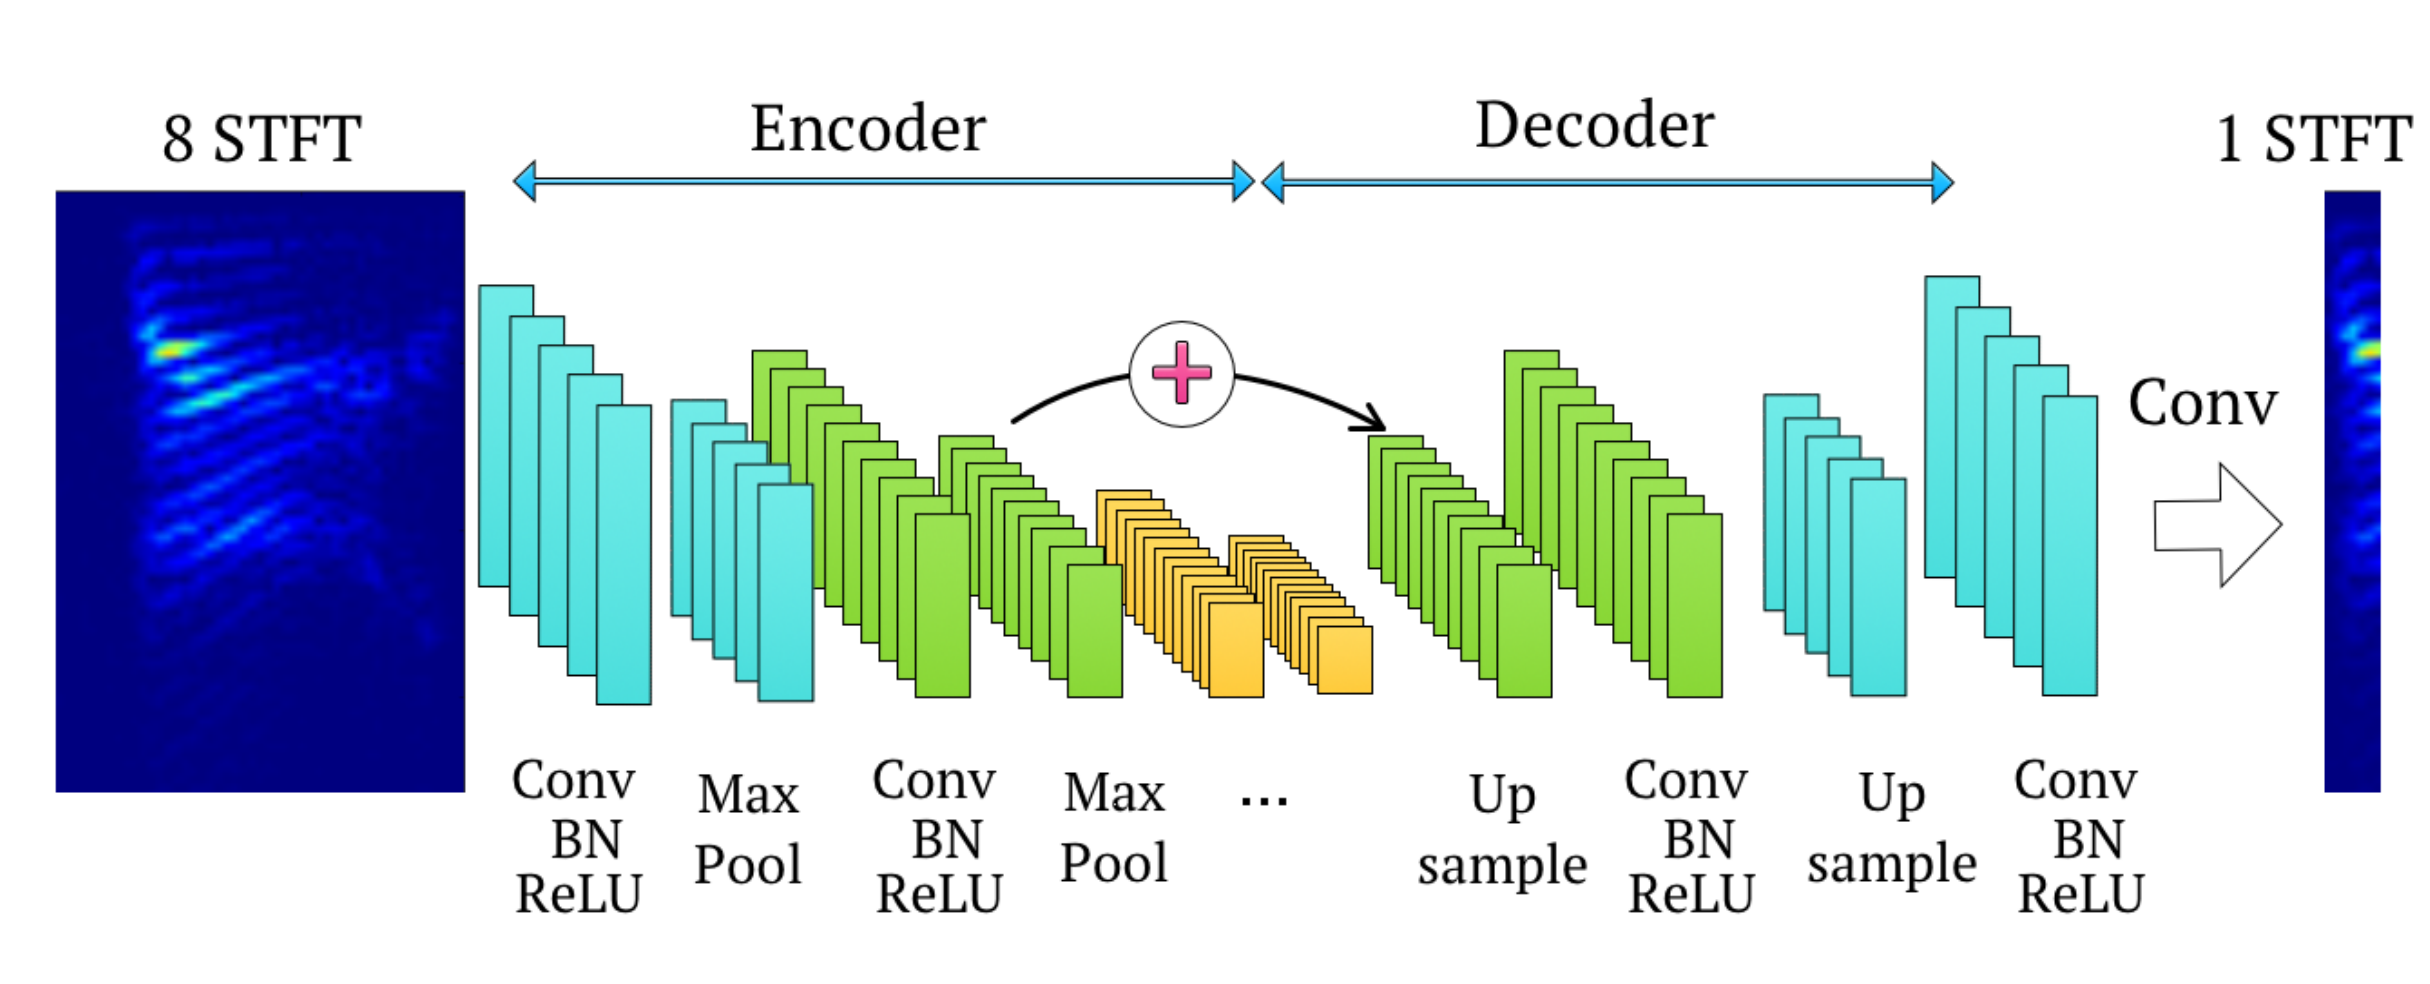
\includegraphics[width=\textwidth,keepaspectratio]{ced.png}
    \caption{\label{fig:ced}Convolutional Encoder Decoder (CED) Network \cite{park2017acoustic}.}
\end{figure}

Unlike the CNN baseline, which includes a dedicated bottleneck to perform feature transformation before decoding, the CED model omits this step entirely. This is because the encoder and decoder in CED are fully connected through the intermediate representation, with no abrupt separation or compression point. As a result, the feature flow between encoding and decoding stages is continuous, allowing for a more gradual and integrated transformation of features across the network. This design is particularly beneficial for temporal structures like speech, where abrupt compression may degrade important patterns.

The decoder mirrors the encoder in structure, using four stages of upsampling followed by convolution, batch normalization, and ReLU activation. Each upsampling layer doubles the temporal dimension using a scale factor of \((2, 1)\), restoring the resolution reduced in the encoder. The decoder reverses the channel progression, reducing from 32 back down to 12. A final convolutional layer with a large vertical kernel of \(129 \times 1\) is used to project the output to two channels, corresponding to the real and imaginary parts of the denoised spectrogram. A bilinear interpolation step is applied at the end to ensure the output matches the original input resolution.

By eliminating the bottleneck and employing deep, temporally-aware convolutional transformations, the CED model enables a smooth and information-preserving mapping from noisy to clean spectrograms. Its symmetric structure, combined with frequency-preserving vertical kernels and temporal downsampling, makes it well-suited for capturing sequential dependencies without sacrificing spectral resolution. In this project, the CED architecture is used as a strong benchmark for assessing the effectiveness of fully convolutional encoder-decoder networks, particularly in contrast to the more compressed representations used in CNN-based designs.

\subsection{Redundant Convolutional Encoder Decoder (R-CED)}
\label{sec:rced}

The Redundant Convolutional Encoder Decoder (R-CED) architecture implemented in this project builds upon the CED framework introduced by Park and Lee~\cite{park2017acoustic} and discussed in Section~\ref{sec:fcns}. Like the CED, R-CED operates on complex spectrograms represented as two-channel inputs (real and imaginary). However, the design omits all pooling and upsampling operations to preserve full temporal and spectral resolution throughout the network.

\begin{figure}[h]
    \centering
    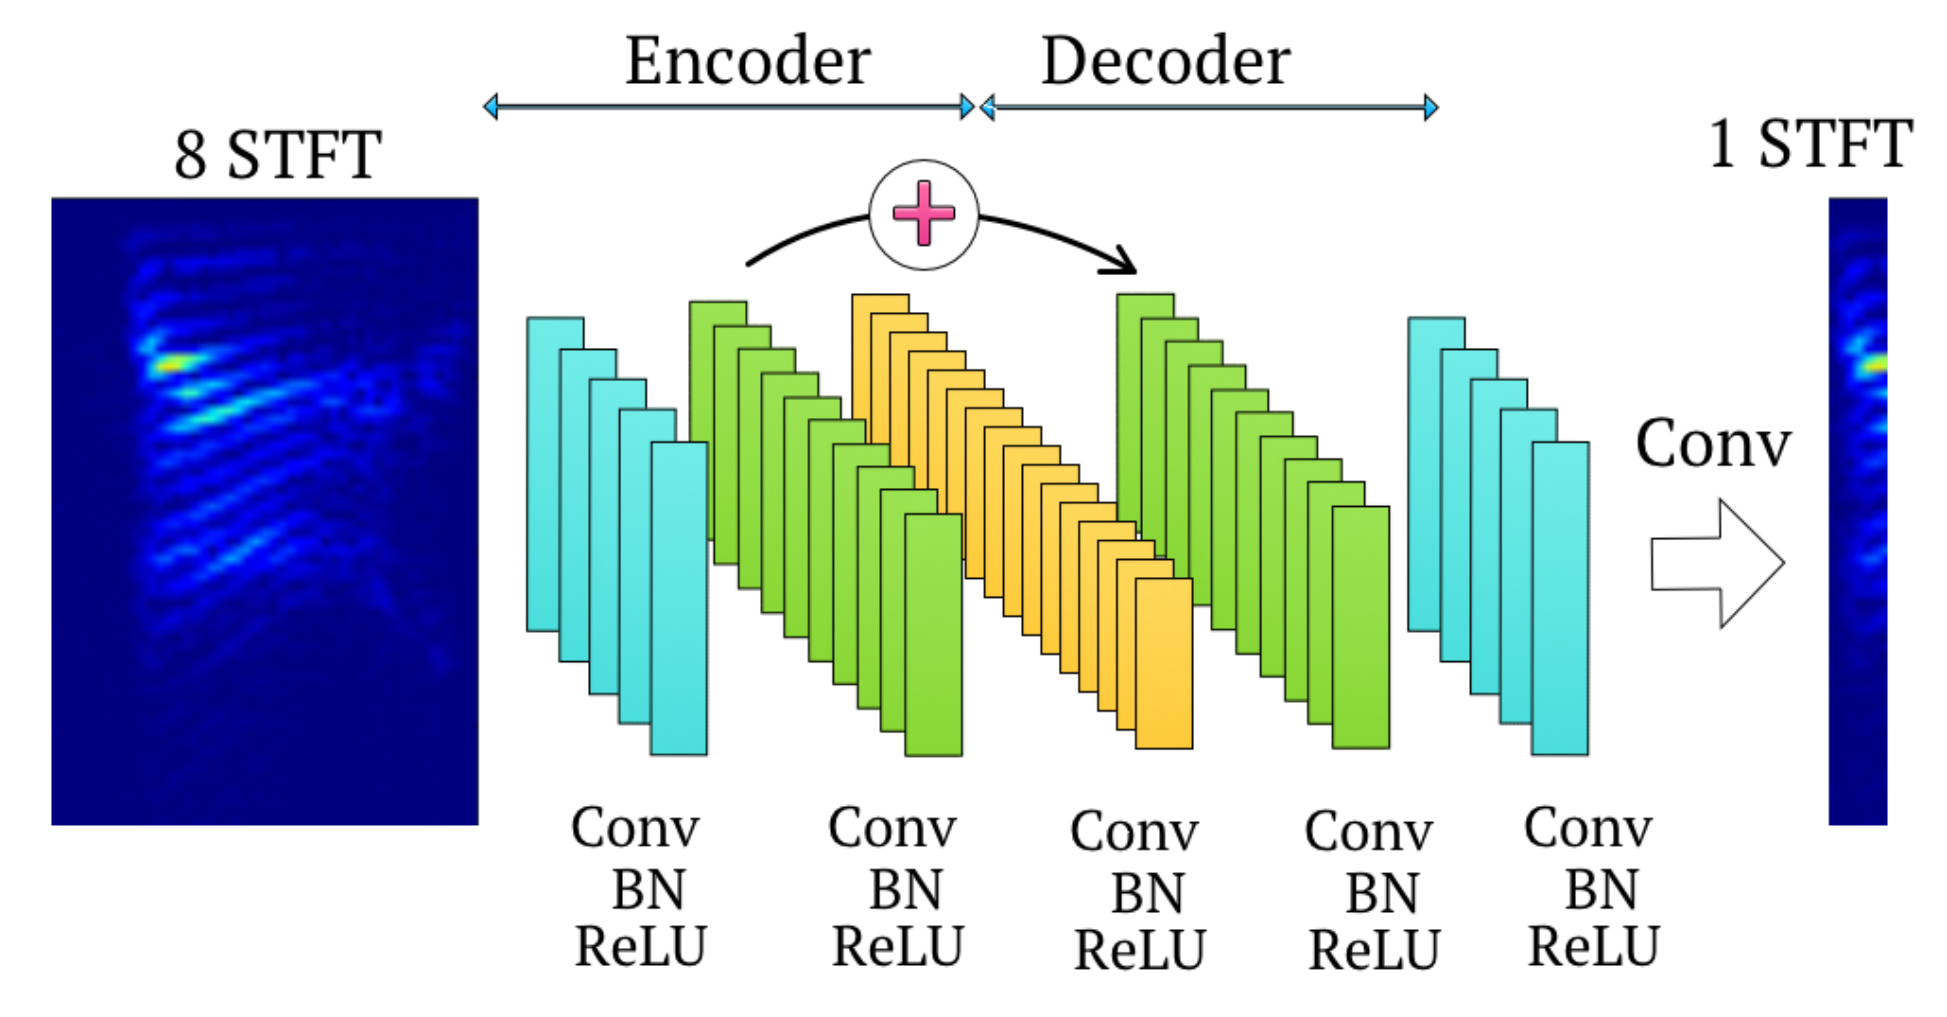
\includegraphics[width=\textwidth,keepaspectratio]{r-ced.png}
    \caption{\label{fig:rced}Redundant Convolutional Encoder Decoder (R-CED) architecture \cite{park2017acoustic}.}
\end{figure}

The network is composed of nine sequential convolutional layers. The first eight layers use tall vertical kernels ranging from \(13 \times 1\) to \(7 \times 1\), symmetrically arranged around the network's midpoint. Each layer is followed by a ReLU activation and batch normalization. The number of channels increases from 2 to 32 in the first half and then mirrors back to 12 in the second half, following the filter progression: 12, 16, 20, 24, 32, 24, 20, 16, 12. This symmetric arrangement enables the model to gradually build and refine feature representations without disrupting the resolution of the input signal.

Unlike typical encoder-decoder models, the R-CED maintains a constant spatial resolution throughout the network. There are no pooling or upsampling layers. Instead, representational depth is increased by stacking more convolutional layers. This redundancy increases the model’s expressive capacity while preserving time-frequency alignment. A crucial property for speech enhancement tasks.

The final convolutional layer uses a \(129 \times 1\) kernel, consistent with the original paper, to project the output down to two channels representing the denoised real and imaginary components. Bilinear interpolation is applied at the end to match the input resolution before output splitting.

By eliminating dimensionality-altering operations and relying on a deeper sequence of convolutional blocks, the R-CED model is able to maintain high-resolution feature representations across all layers. This architecture is especially useful in applications where preserving the fine structure of spectrograms is essential. In this project, R-CED is evaluated as a resolution-preserving alternative to encoder-decoder architectures, providing a balance between simplicity and performance.

\subsection{U-Net}
\label{sec:unet}

The U-Net model implemented in this project is adapted from the widely known U-Net architecture originally proposed for biomedical image segmentation~\cite{ronneberger2015unet}. In this work, it is repurposed for the task of speech enhancement using complex spectrograms. The model follows a symmetric encoder-decoder structure with skip connections and is designed to recover clean speech signals by operating directly on the concatenated real and imaginary spectrogram components.

The encoder consists of five convolutional blocks, each followed by instance normalization and a PReLU activation. Downsampling is achieved by using a stride of 2 in all but the first convolution block. The channel depth increases progressively from 2 to 1024 across the five stages: \(2 \rightarrow 64 \rightarrow 128 \rightarrow 256 \rightarrow 512 \rightarrow 1024\). Instance normalization is preferred over batch normalization for improved stability with variable-length or low-batch-size audio inputs.

\begin{figure}[h]
    \centering
    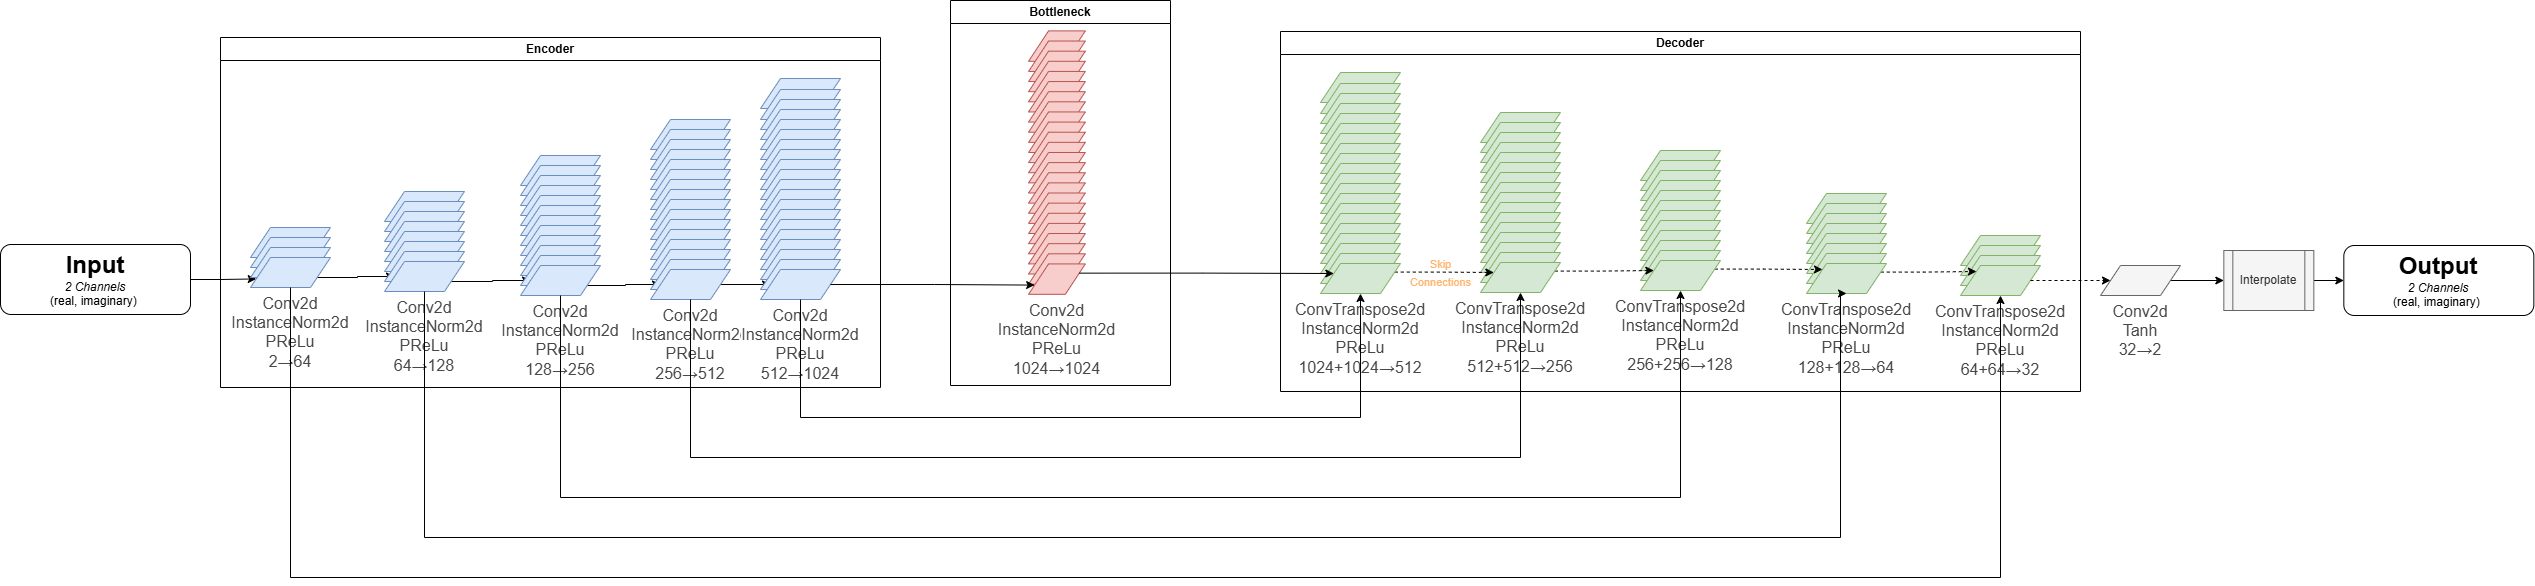
\includegraphics[width=\textwidth]{unet.png}
    \caption{\label{fig:unet}U-Net Architecture.}
\end{figure}

At the center of the network is a bottleneck block that maintains the 1024-channel depth while applying an additional convolution, instance normalization, and PReLU activation. Unlike traditional bottlenecks that compress the latent representation, this layer serves as a non-linear transformation hub that enhances the feature space before decoding.

The decoder mirrors the encoder in structure, consisting of five transposed convolutional blocks that progressively upsample the feature maps and reduce channel depth. At each stage, features from the corresponding encoder block are concatenated with the upsampled decoder output via skip connections. Since downsampling in the encoder affects spatial resolution, bilinear interpolation is used to resize encoder features before concatenation to ensure dimensional alignment.

The decoder proceeds through five stages of channel reduction: \(1024 \rightarrow 512 \rightarrow 256 \rightarrow 128 \rightarrow 64 \rightarrow 32\), followed by a final \(3 \times 3\) convolutional layer projecting to 2 output channels corresponding to the real and imaginary parts of the denoised spectrogram. A final bilinear interpolation step ensures that the output resolution matches the original input dimensions.

This U-Net implementation preserves the architectural strengths of the original model while tailoring its structure for speech enhancement. The use of skip connections, instance normalization, and a deep encoder-decoder hierarchy enhances the model’s ability to recover spectro-temporal structure, making it a powerful architecture for complex denoising tasks.

\subsection{Conv-TasNet}
\label{sec:convtasnet}

The Conv-TasNet model implemented in this project is based on the architecture proposed by Luo and Mesgarani~\cite{luo2019conv}, as discussed in Section~\ref{sec:convtasnet_lit_review}. Although the core structure is preserved, several adaptations were made to align the model with the spectrogram-based input framework used throughout this system.

The original Conv-TasNet operates directly on time-domain audio signals. In contrast, this implementation modifies the input format to handle complex-valued spectrograms. The real and imaginary components are concatenated along the channel dimension, forming a two-channel input that is passed through a \(3 \times 3\) convolutional encoder. The encoder expands the input to a latent space with 128 channels using dynamic padding to preserve the original time-frequency resolution.

\begin{figure}[h]
    \centering
    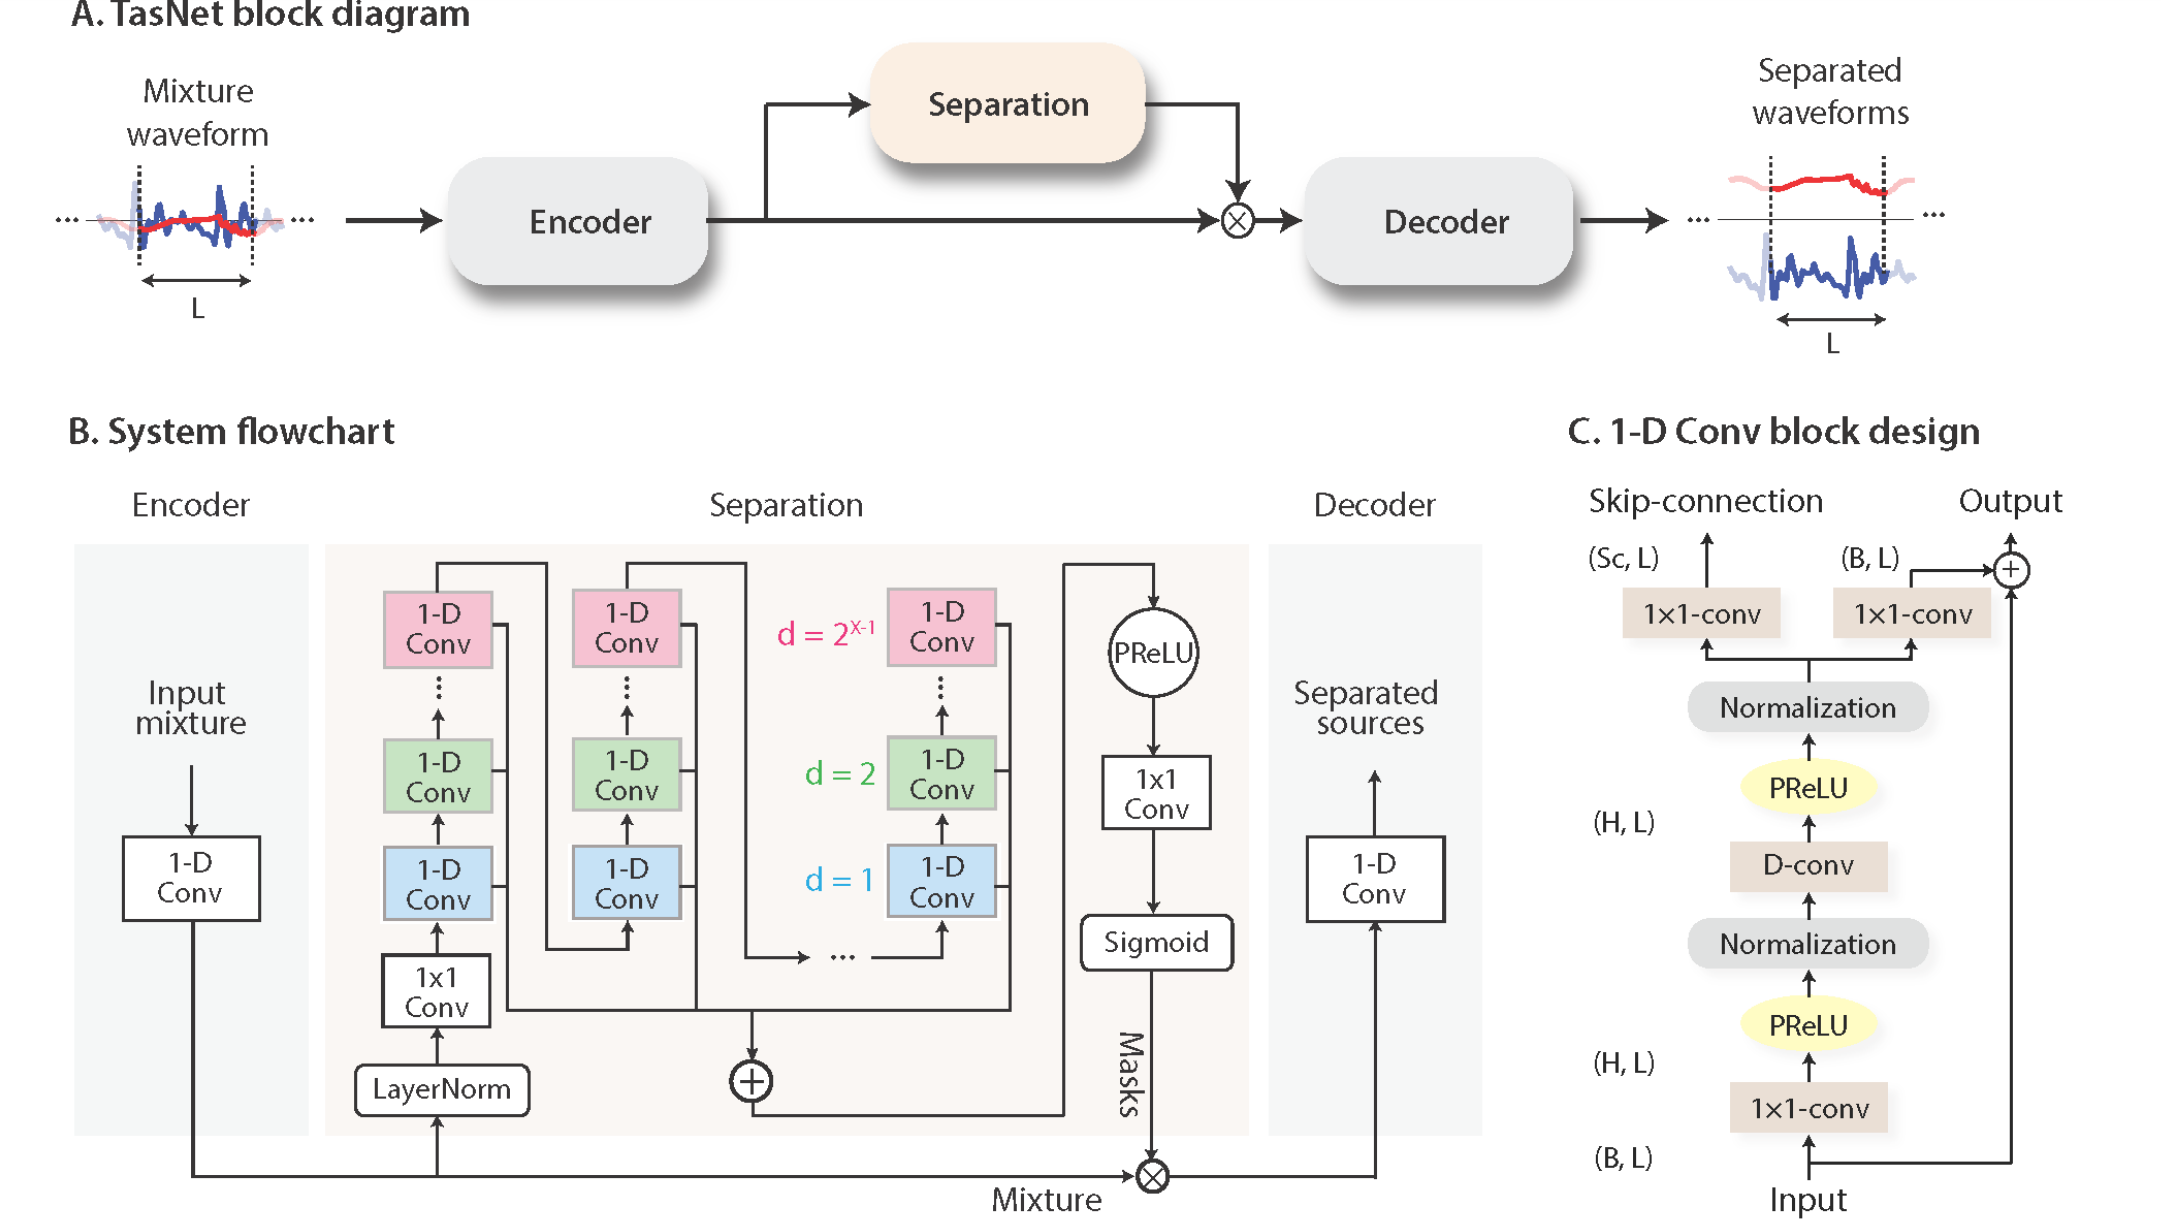
\includegraphics[width=\textwidth,keepaspectratio]{conv-tasnet.png}
    \caption{\label{fig:convtasnet}Conv-TasNet architecture overview \cite{luo2019conv}.}
\end{figure}

The encoded features are passed to a Temporal Convolutional Network (TCN), which serves as the core separation module. The TCN is composed of two stacks, each containing four residual blocks, for a total of eight layers. Each residual block consists of a dilated convolution with exponentially increasing dilation factors (e.g., 1, 2, 4, 8), followed by group normalization (with eight groups), a PReLU activation, and a second projection convolution. A residual connection is used to stabilize training and preserve input information. The dilation strategy allows the TCN to model long-range temporal dependencies efficiently while maintaining a fixed receptive field size.

Unlike the original Conv-TasNet, which applies explicit time-domain masking for source separation, this implementation omits masking altogether. Instead, the TCN directly outputs an enhanced latent representation, which is then decoded into denoised real and imaginary spectrogram components via a final \(3 \times 3\) convolutional layer. This choice simplifies the architecture and reduces overhead, as preliminary testing showed only marginal performance gains from complex masking.

The output of the decoder is aligned with the original input size by cropping along both frequency and time axes to correct for minor size mismatches introduced by convolutional operations. This ensures a consistent dimensionality before inverse STFT reconstruction.

By preserving the temporal modeling strength of the original TCN structure and adapting it to operate in the complex spectrogram domain, this implementation of Conv-TasNet offers a powerful yet flexible architecture for speech denoising. It combines deep receptive fields, efficient convolutional modeling, and skip connections within residual blocks to robustly recover clean speech across variable-length inputs.

\vspace{2em}
This project explores a range of neural network architectures for speech enhancement, beginning with a simple CNN-based autoencoder as a baseline. It then progresses to fully convolutional models such as the Convolutional Encoder Decoder (CED) and its redundant variant, R-CED, both derived from the work of Park and Lee~\cite{park2017acoustic}. The U-Net architecture further improves performance through the use of skip connections and a deeper encoder-decoder structure. Finally, Conv-TasNet~\cite{luo2019conv}, originally developed for speech separation in the time domain, is adapted for spectrogram-based denoising by leveraging its powerful Temporal Convolutional Network (TCN). Together, these models offer a diverse and comparative landscape of deep learning approaches, highlighting architectural trade-offs and establishing strong baselines for benchmarking against classical signal processing techniques.


